\documentclass[11pt,a4paper]{article}
\usepackage[margin=1in]{geometry}
\usepackage[T1]{fontenc}
\usepackage[utf8]{inputenc}
\usepackage{lmodern}
\usepackage{hyperref}
\usepackage{enumitem}
\usepackage{xurl}
\usepackage{tikz}
\usepackage{float}
\usetikzlibrary{arrows.meta, positioning, shapes.geometric}
\hypersetup{colorlinks=true,linkcolor=blue,urlcolor=blue}
\newcommand{\codepath}[1]{\path{#1}}
\tikzset{box/.style={rectangle,draw,rounded corners,align=center,inner sep=3pt,minimum width=36mm},line/.style={-Latex}}

\title{Phase-1 Deliverable: CLI Pipeline}
\author{SIT Engine Architecture}
\date{\today}

\begin{document}
\maketitle

\section{Technical Description}
CLI Pipeline is the developer-facing execution surface for deterministic staged runs: ingest \(\rightarrow\) classify \(\rightarrow\) export.

\section{Implementation Fulfillment}
Implemented in \codepath{Phase-1/cli.py} with \texttt{cmd\_ingest}, \texttt{cmd\_classify}, and \texttt{cmd\_export}. Packaging entrypoint is declared in \codepath{Phase-1/pyproject.toml} as \texttt{riscvbench}.

\section{Design \& Architecture}
Stage boundaries are file-backed (manifest, trace, windows, summary, export) for reproducibility, debug visibility, and CI stage decomposition.

\subsection*{Function Flowchart}
\begin{figure}[H]
\centering
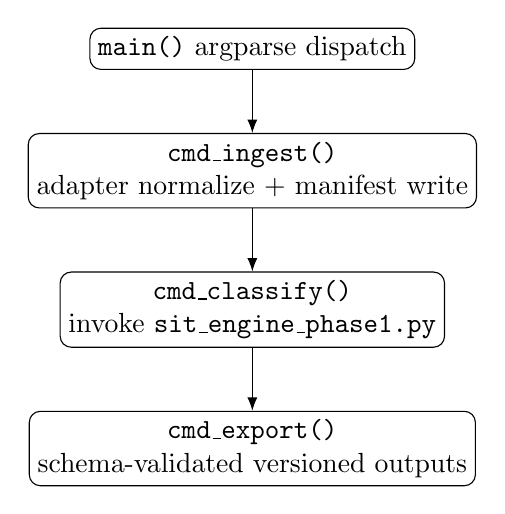
\begin{tikzpicture}[node distance=8mm and 12mm]
\node[box] (a) {\texttt{main()} argparse dispatch};
\node[box, below=of a] (b) {\texttt{cmd\_ingest()}\\adapter normalize + manifest write};
\node[box, below=of b] (c) {\texttt{cmd\_classify()}\\invoke \texttt{sit\_engine\_phase1.py}};
\node[box, below=of c] (d) {\texttt{cmd\_export()}\\schema-validated versioned outputs};
\draw[line] (a) -- (b);
\draw[line] (b) -- (c);
\draw[line] (c) -- (d);
\end{tikzpicture}
\caption{CLI Pipeline Function Flow}
\end{figure}

\end{document}
